\documentclass[assignment07_Solutions]{subfiles}

\invalidatemargin

\IfSubStr{\jobname}{\detokenize{Solutions}}{\toggletrue{solutions}}{\toggletrue{solutions}}

%\IfSubStr{\jobname}{\detokenize{Solutions}}{\toggletrue{solutions}}{\togglefalse{solutions}}

\fancypagestyle{firstpage}

{\rhead{Assignment 7 \linebreak \textit{Version: \today}}}

\title{Assignment 7: Pytorch, Vanishing Gradients, and Convolutional Neural Networks}
\author{Machine Learning}
\date{Fall 2019}

\begin{document}

\maketitle
\thispagestyle{firstpage}


\begin{learningobjectives}
\bi
\item Learn the basics of Pytorch
\item Understand the vanishing gradient problem and how to fix it
\item Learn about convolutional neural networks from a conceptual perspective
\item Apply convolutional neural networks to a real dataset.
\ei
\end{learningobjectives}

\begin{priorknowledge}
\bi
\item Multilayer perceptron
\item Backpropagation
\ei
\end{priorknowledge}

\section{Pytorch and Autograd Algorithms}

In this assignment you will be learning about another new Python library: pytorch.  \href{https://pytorch.org/}{Pytorch} is an open-source library designed for high-performance machine learning.  There are a number of other similar frameworks out there.  We chose pytorch due to its straightforward data handling, flexibility, and support for debugging.  Below, we'll list two other frameworks and why we, ultimately, decided to go with pytorch.

\bi
\item \href{https://keras.io/}{Keras} also lets you construct high-performance neural networks in Python.  The biggest downside in our eyes is that it hides away a lot of the details of how data moves through the network making it a bit too abstract for our purposes (e.g., harder to debug and less flexible).
\item \href{https://www.tensorflow.org/}{TensorFlow} is another package that is similar to pytorch.  Tensorflow is more popular than pytorch, but it is a bit more complicated and has a steeper learning curve than pytorch.
\item sklearn has support for Multilayer Perceptrons (as we saw in the last notebook).  That said it doesn't support very many sorts of networks and it doesn't support high performance computation using GPUs (graphics processing units).
\item numpy would also be an option.  It is very flexible, but too low-level and like sklearn doesn't support high performance computation with GPUs.
\ei

Before we have you start going through some resources on how to use pytorch, let's discuss what we are hoping to get from pytorch.
\bi
\item The ability to automatically compute gradients of our model parameters with respect to our loss function!
\item The ability to run our neural network on a GPU (for performance boosts of up to 20 times).
\item Tools for debugging common problems with neural networks.
\item A module called torchvision for working with images in neural networks.
\ei

Go through the following tutorials for pytorch.  This will give you the barebones and then we'll follow that up with a little bit later in this document with our own companion notebooks that will help you get even more familiar with pytorch.
\begin{externalresources}
We recommend you go through these with Colab open so you can try the blocks of code yourself.
\bi
\item \href{https://pytorch.org/tutorials/beginner/blitz/tensor_tutorial.html}{Tensor Tutorial} (\href{http://nb.mit.edu/f/55481}{on NB})
\item \href{https://pytorch.org/tutorials/beginner/blitz/autograd_tutorial.html}{Autograd Tutorial} (\href{http://nb.mit.edu/f/55482}{on NB})
\ei
\end{externalresources}



\section{Backpropagation and the Problem of Vanishing (or Exploding) Gradients}
One possible reaction to reading about the autograd capabilities in pytorch is to think ``Why didn't Paul and Sam tell me about this before?  Why have we been wasting our time doing all this math to compute gradients?''  There are really two (in our opinion) good answers to this line of questions.
\be
\item Knowing the algorithm (backpropagation) for computing the gradient gives you a more powerful mental model of how these networks are trained, how to diagnose failures in training, and potentially how to fix these failures.
\item The math you learned along the way was super useful even outside of machine learning.
\ee

One particularly important version of point 1 above is known as the vanishing gradient problem (or its more dramatic sounding counterpart the exploding gradient problem).  You'll be reading all about it in just a bit, but before we dive in let's review the multi-layer perceptron (MLP).

\begin{recall}[Multi-layer perceptron]
The multi-layer perceptron consists of a bunch of single-layer perceptrons stacked on top of each other.  Last assignment we saw a particular special case of this where we just a few logistic regression models and stack them.  A cartoon version of the network applied to the titanic dataset is shown below.

\begin{center}
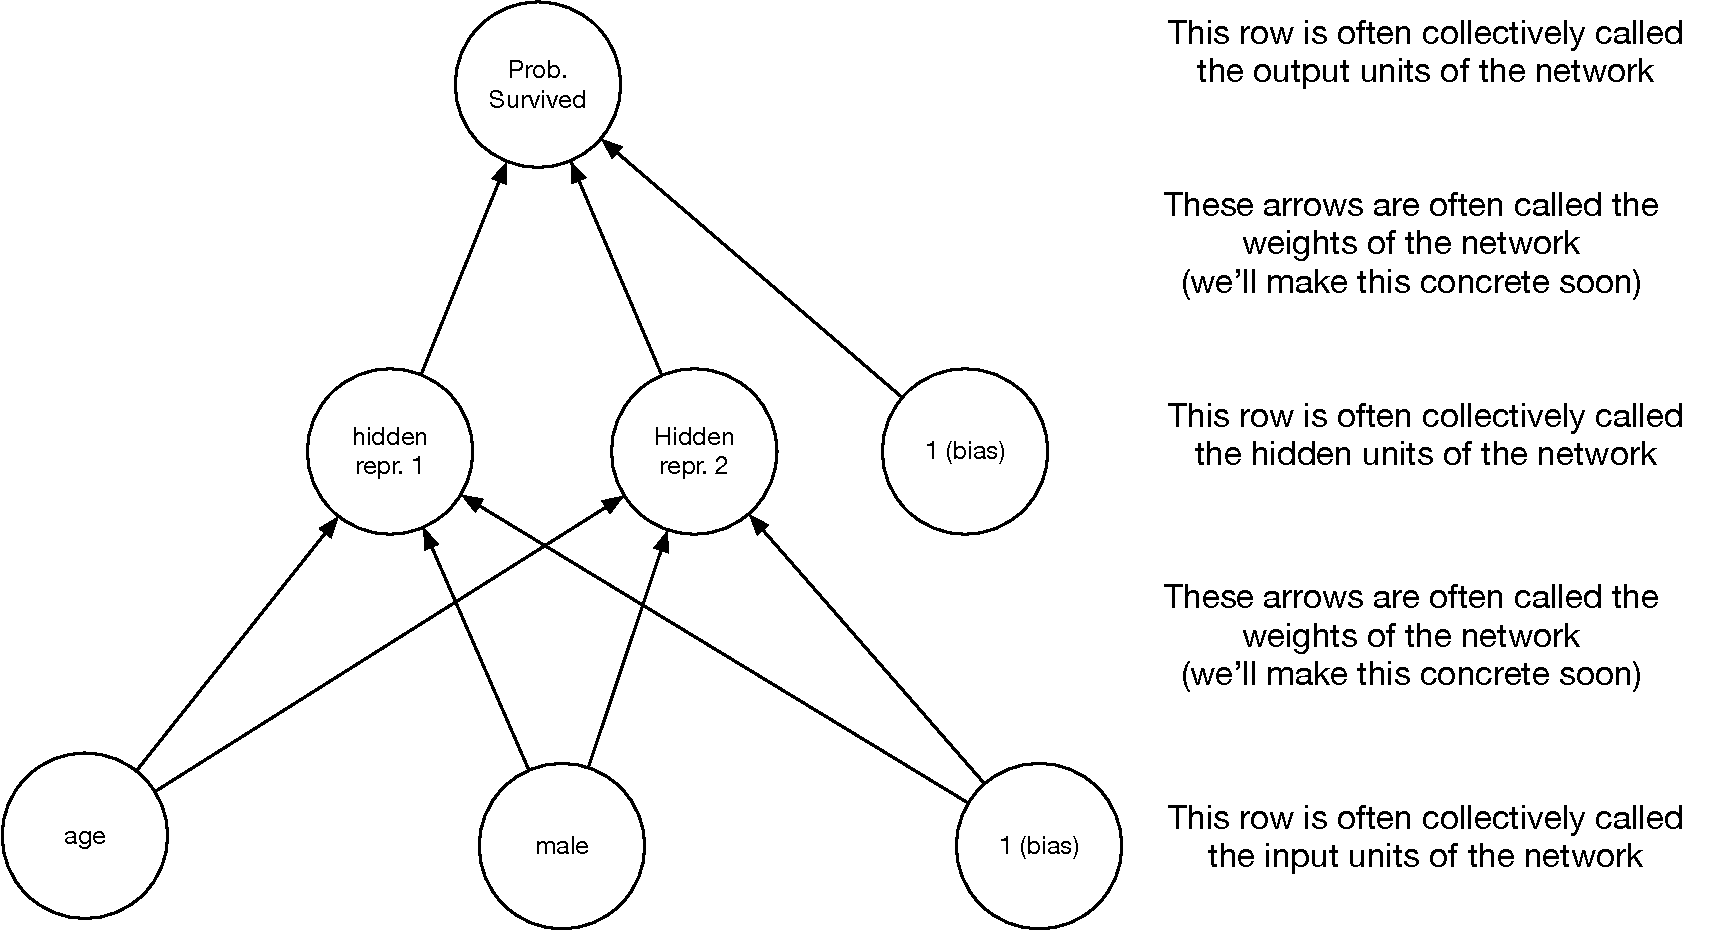
\includegraphics[width=0.7\linewidth]{figures/titanicmlpsimple}
\end{center}

We saw in the companion notebook what such networks are capable of (e.g., learning useful internal representations for prediction).  To make the figure above even more precise, we can zoom in on how data propagates from lower layers to higher layers in the network (view 1 in the figure below) and ultimately to the loss function (view 2 in the figure below).

\vspace{1em}

For your convenience, here is a notation guide for this figure that is to follow.
\vspace{1em}

\begin{tabular}{| c | l |}
\hline
$l$ & the loss function for the network (log loss in this case) \\
\hline
$m$ & the number of layers in the network \\
\hline
$n_{k}$ & the number of nodes in the $k$th layer \\
\hline
$x_j^{(k)}$& The $j$th node in the $k$th layer of the network ($k = 1$ is the input \\
&and $k = m$ is the output) \\
\hline
$\mathbf{x^{(k)}}$ & The nodes at the $k$th layer in vector form \\
\hline
$s_{i}^{(k)}$ & the $i$th summation node in the $k$th layer \\
\hline
$w_{i,j}^{(k)}$ & the weight connecting the $j$th node in layer k to the $i$th node in\\
&  layer $k+1$ \\
\hline
$\mlvec{w_{i}^{(k)}}$ & the vector of weights to the $i$th summation node in layer $k+1$.\\
\hline
\end{tabular}

\begin{center}
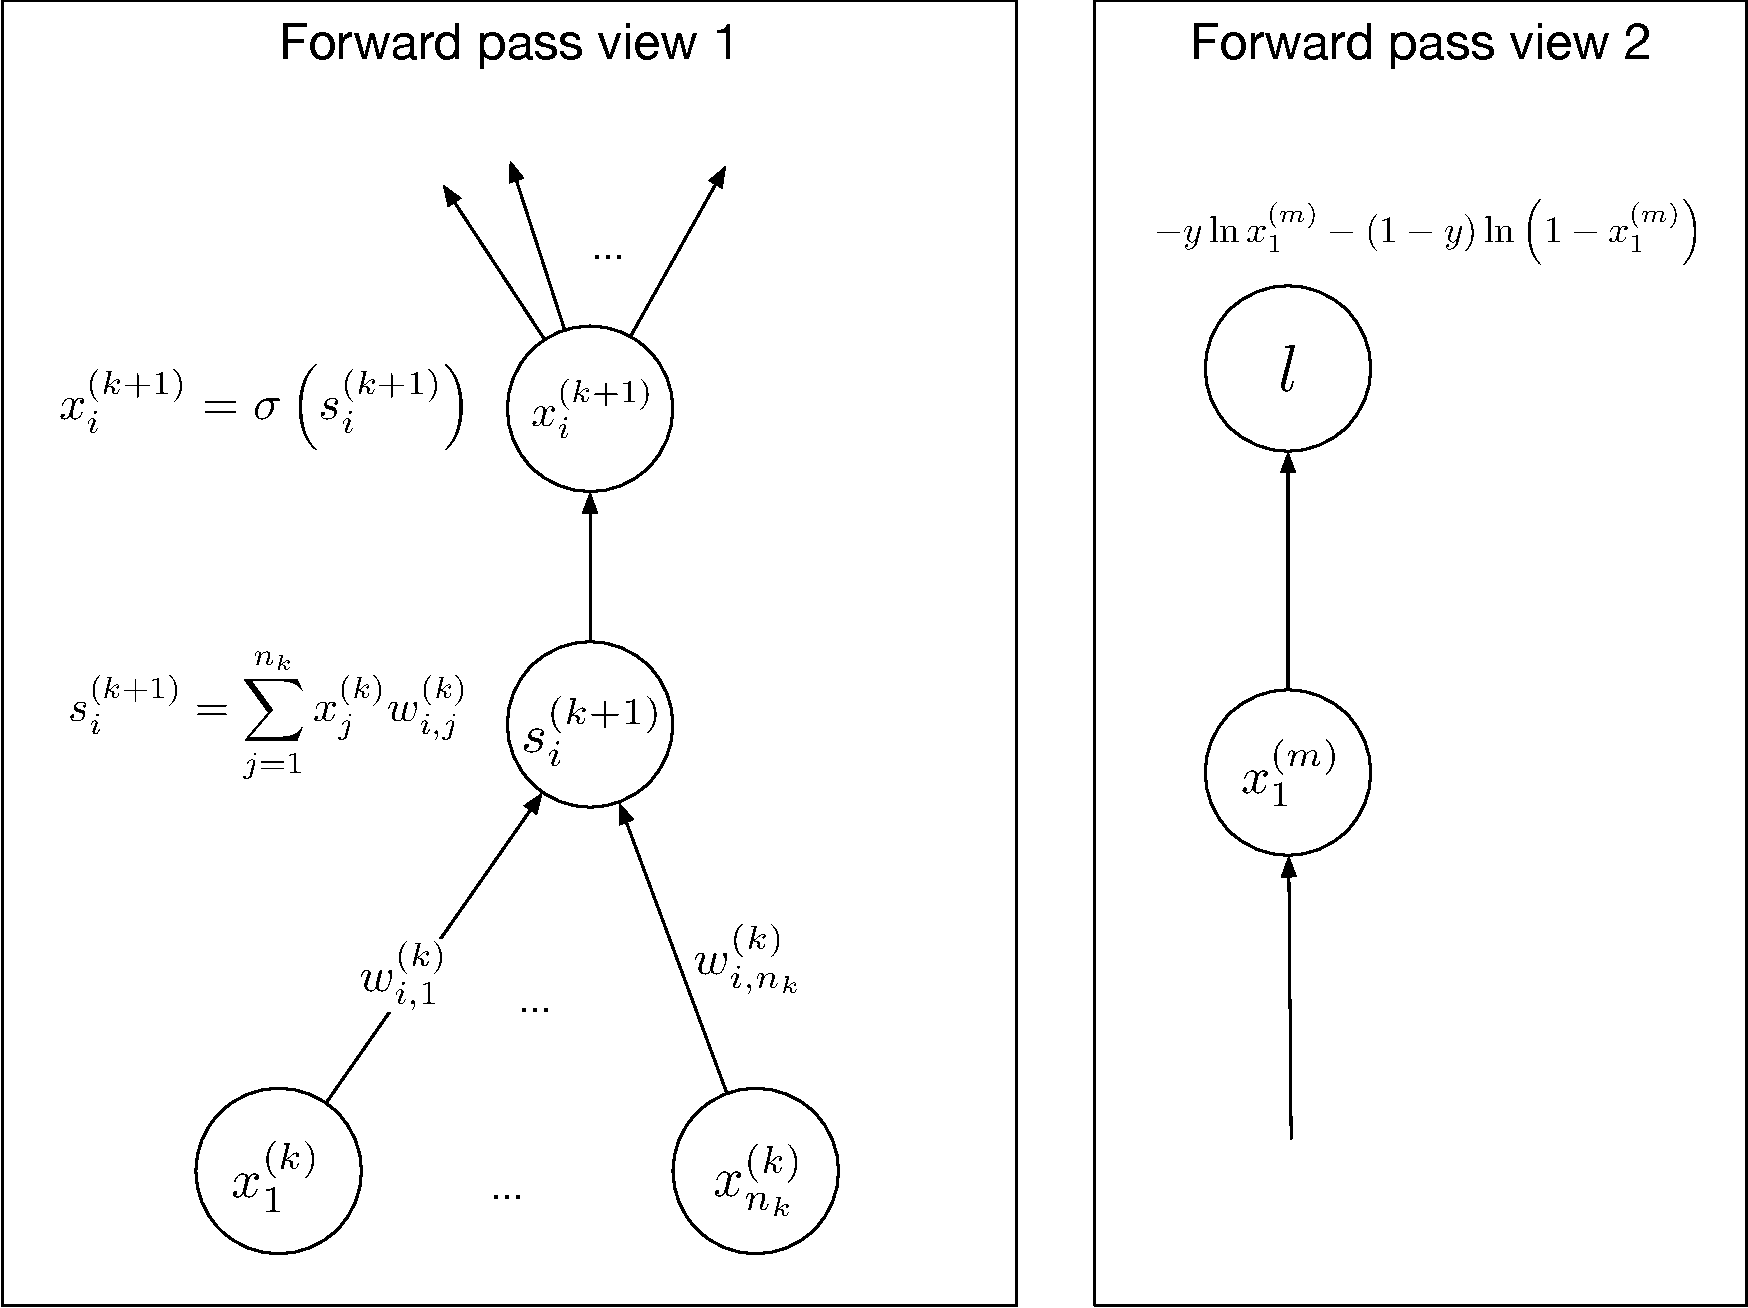
\includegraphics[width=0.7\linewidth]{figures/mlpfullforward}
\end{center}

\end{recall}

In the previous assignment you derived the backpropagation algorithm, which can be used to compute the gradient of the weights in an MLP with respect to the loss function.  What's beautiful about this formula is that it works for networks of arbitrary depth.  You may have heard of \href{https://en.wikipedia.org/wiki/Deep_learning}{deep learning}, which is where networks of dozens or even hundreds of layers are trained on a particular task.  Despite their complexity, these networks are typically trained using the backpropagation algorithm you met in the last assignment!

Despite the relative simplicity of the backpropagation equations, there are some dangers lurking when applying the algorithm to deep networks ($m$ very large).  The most common pitfalls that one encounters are \textbf{vanishing and exploding gradients}.  A vanishing gradient is when the gradient of the loss with respect to the weights in a layer becomes vanishingly small as you move from the output layer back towards the input layer.  An exploding gradient is the opposite problem (when the gradient of the loss with respect to the weights in a layer becomes exceedingly large as you move from the output layer towards the input layer).

\begin{exercise}[(60 minutes) or (120 minutes including optional part)]
Before starting this exercise, go and learn about the vanishing gradient problem.  Here are a few resources to look at.  You do not need to read all of them, so please pick the ones that seem the most inline with how you learn.
\begin{externalresources}
\bi
\item \href{https://ayearofai.com/rohan-4-the-vanishing-gradient-problem-ec68f76ffb9b}{Rohan Kapur's Intuitive Explanation of the Vanishing Gradient Problem} (\href{http://nb.mit.edu/f/55483}{on NB})
\item Video resource: \href{https://www.youtube.com/watch?v=SKMpmAOUa2Q}{Deep Learning Simplified: An Old Problem}
\ei
\end{externalresources}


Last assignment we derived the following backpropagation equations.

\begin{align}
(\nabla_{\mathbf{w^{(k)}_i}}) l &= \mlvec{x^{(k)}} \sigma\left (s_i^{(k+1)} \right )\left (1-\sigma\left (s_i^{(k+1)} \right )\right) \frac{\partial l}{\partial x_i^{(k+1)}} & \mbox{gives us the gradient of the weights going into a unit} \\
\frac{\partial l}{\partial x^{(k)}_i} &= \sum_{j=1}^{n_{k+1}} w^{(k)}_{j,i} \sigma \left ( s_{j}^{k+1} \right) \left (1-\sigma \left ( s_{j}^{k+1} \right)\right) \frac{\partial l}{\partial x^{(k+1)}_j} \label{eq:recursion} & \mbox{recursively gives the partial of the loss w.r.t. the units} \\
\frac{\partial l}{\partial x^{(m)}_1} &= -y\frac{1}{x_1^{m}} + (1-y) \frac{1}{1-x_1^{(m)}} & \mbox{provides the base case of the recursion}
\end{align}

\bes
\item If we examine these equations, we can understand much better where the vanishing gradient problem comes from.  In particular, Equation~\ref{eq:recursion} provides the crucial recursive formula for defining the partial derivatives of the loss with respect to nodes in the network in terms of the same partial derivatives for nodes deeper in the network (i.e., closer to the output).  Based on Equation~\ref{eq:recursion}, what aspects of the network might contribute to or counteract the vanishing gradient problem? Consider things such as the values of the summation units $s_j^{(k+1)}$, the values of the weights, and the number of units at each layer of the network (the $n_k$'s).
\item It turns out that the sigmoid function is only one viable choice for transforming the summation units into the values of the units for the next layer.  In fact, many different  non-linear functions can be used (e.g., \href{http://mathworld.wolfram.com/HyperbolicTangent.html}{tanh}).  The function used in this capacity is called an \emph{activation function}.  If we let $a$ refer to our activation function, then Equation~\ref{eq:recursion} becomes

\begin{align}
\frac{\partial l}{\partial x^{(k)}_i} &= \sum_{j=1}^{n_{k+1}} w^{(k)}_{j,i} a' \left ( s_{j}^{k+1} \right)  \frac{\partial l}{\partial x^{(k+1)}_j} \label{eq:recursion2} \enspace .
\end{align}


One very popular choice of activation function is called \href{https://en.wikipedia.org/wiki/Rectifier_(neural_networks)}{rectified linear} (or ReLu for \emph{rectified linear unit}).  A graph of the ReLu activation function is shown below.

\begin{center}
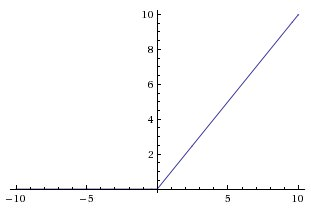
\includegraphics[width=0.4\linewidth]{figures/relu}
\end{center}

How might choosing the ReLu as an activation function help with the vanishing gradient problem in comparison to choosing the sigmoid as your activation function?

\item \textbf{Going Beyond (optional)} Using pytorch, perform a computational investigation of the vanishing gradient problem.  We suggest the following steps (note: we have our own version of this in the solutions if you want to check it out):
\bi
\item Create an MLP where the number of layers is passed in as a parameter.
\item Before doing any training of the network, feed an arbitrary input into the network, compute the loss, and then compute the gradient of the loss with respect to the weights at each level of the network.
\item Summarize the partial derivatives of the weights at each level in the network (e.g., take the mean of the absolute values) and plot this quantity as a function of $k$ (the layer number).  It may be helpful to use a log scale for the y-axis.
\ei
\ees

\end{exercise}

\section{Convolutions and Image Filtering}

Depending on your math background you may have seen the convolution operation before.  There are various types of convolutions, including convolutions with continuous functions, discrete functions, in 1d, in 2d, or in higher dimensions.  In this class we're only going to be talking about 2D convolutions.  It turns out that such convolutions provide a compelling way to think about processing data with intrinsically 2D structure (such as images).

Check out at least one of the resources below to learn how convolutions can be used to filter and transform images.

\begin{externalresources}[(30 minutes)]
\bi
\item \href{http://machinelearninguru.com/computer_vision/basics/convolution/image_convolution_1.html}{Image Filtering} (\href{http://nb.mit.edu/f/55484}{on NB})
\item Video resource: \href{https://www.youtube.com/watch?v=C_zFhWdM4ic}{How blurs and filters work}
\ei
\end{externalresources}

\begin{exercise}
Check understanding.

\bes
\item f
\ees
\end{exercise}


\section{Convolutional Neural Networks}
We now come to a particular type of neural network called a convolutional neural network.  These networks supplement the perceptron layers we've seen thus far with convolutional layers that apply various filtering operations to the data.  These networks are very well-suited for working with images since they are able to customize their filtering operations to the dataset in a way that maximizes their ability to solve the task.  There are lots of great resources on convolutional neural networks out there.  Please don't feel like you have to go through all of these.

\begin{externalresources}[(60 minutes)]
\bi
\item \href{https://ujjwalkarn.me/2016/08/11/intuitive-explanation-convnets/}{Intuitive Explanation of Convnets} (\href{http://nb.mit.edu/f/55489}{on NB}) (this one is a very well done high-level overview)
\item \href{http://scs.ryerson.ca/~aharley/vis/conv/flat.html}{Beautiful interactive visualization of a Convnet trained to recognize handwritten digits} (this is great, especially for visual learners.  Make sure to click on the activations at a layer to see the learned filter.  Don't miss this one!)
\item \href{https://cs.stanford.edu/people/karpathy/convnetjs/}{Convnet.js} (convnets training in your browser?!? Another good one for visual learners)
\item \href{https://www.datascience.com/blog/convolutional-neural-network}{Convolutional Neural Networks Explained} (\href{http://nb.mit.edu/f/55488}{on NB}) (this one is quite similar to the ``intuitive explanation of convnets.''  It's a little shorter though.)
\item \href{https://www.youtube.com/watch?v=bNb2fEVKeEo&list=PL3FW7Lu3i5JvHM8ljYj-zLfQRF3EO8sYv\&index=5}{Lecture 5 from CS231 at Stanford} (if you want a lecture, this one is good.  it starts getting a bit too low-level around the 35 minute mark.  there are some nice slides on neural network history at the beginning).
\ei
\end{externalresources}

\begin{exercise}
Check understanding.

\bes
\item TODO
\ees
\end{exercise}

\section{Training Your First Convnet}

TODO: NINJAs to work on this.

\section{Something on Context and Ethics and Convnets (if we pushed project out another day, I would vote for this}

\section{Getting Ready for the Project}
Sam to work on this.
\subsection{Goals}
\subsection{Datasets}

\end{document}
